\documentclass[oneside,a4paper,11pt,explicit]{book}
\usepackage[utf8]{inputenc}
\usepackage{icecream}
\usepackage[english]{babel}
\addto\captionsenglish{\renewcommand{\chaptername}{}}
\usepackage[accsupp]{axessibility}  % improves PDF readability for those with disabilities.
\usepackage[colorlinks = true,urlcolor  = blue,linkcolor = blue]{hyperref}
\usepackage{setspace}
\usepackage{listings}
\usepackage[most]{tcolorbox}
\usepackage{minitoc}


\renewcommand{\mtifont}{\large\sffamily}
\renewcommand{\mtcfont}{\small\sffamily}
\renewcommand{\mtcSfont}{\small\sffamily}
\renewcommand{\mtcSSfont}{\small\sffamily}
\renewcommand{\mtcSSSfont}{\small\sffamily}
\mtcsetpagenumbers{minitoc}{off} % turn off page numbering in minitocs
\addto{\captionsenglish}{% Making babel aware of special titles
	\renewcommand{\mtctitle}{Quick Links To Sections}
}
\setlength{\fboxrule}{5pt}
\setlength{\fboxsep}{4pt}

\definecolor{IceCreamLeaf}{rgb}{0.4, 0.639215686274, 0.4}
\definecolor{IceCreamOrbit}{rgb}{0.803921568627451, 0.3607843137254902, 0.3607843137254902}

\pretolerance=10000
\tolerance=2000 
\emergencystretch=10pt

%%%%%%%%%%%%%%% END PREAMBLE

\title{I.C.E.C.R.E.A.M. Tutorials}
\subtitle{\small Observing Earth from Above (Env 329) v24.06 \\
	\small Schmid College of Science and Technology, Chapman University}
\date{\today}

%% DOCUMENT
\setstretch{1.25}
\makeatletter
\begin{document}
	
	\dominitoc
	
	%\tableofcontents
	
	\setcounter{chapter}{7} %Insert (Tutorial Number-1) Here; example for tutorial 4, enter 3
	
	\chapter{Hometown Temperature Competition} %Enter Tutorial Name Here
	
	\vspace{-2em}
	
	\minitoc
	
	\hrule
	
	\vspace{1em}
	
	\begin{tcolorbox}[enhanced,frame style image=blueshade.png,
		opacityback=0.75,opacitybacktitle=0.25,
		colback=blue!5!white,colframe=blue!75!black,title={\Large \textbf{Objectives:}}]
		\large
		\begin{enumerate}
			\item Access and download land surface data from ECOSTRESS of the highest and lowest temperatures in 2022 for your hometown or favorite place you have lived.
			\item Create a map that easily communicates this information. 
			\item See who's hometown is the hottest and coldest!
		\end{enumerate}
	\end{tcolorbox}
	
	\clearpage
	
	%%%%%%%%%%%%%%%%%%%%%%%%%%%%%%%%%% Change Header to Have a Smaller Logo for Remainder of the Document
	\fancyhead{}
	\fancyhead[C]{\begin{tikzpicture}[overlay, remember picture]
			\fill[Blue2] (current page.north west) rectangle ($(current page.north east)+(0,-1in)$);
			\node[anchor=north west, text=white, font=\Large, minimum size=1in, inner xsep=5mm, align=left] at (current page.north west) {\bf{\MakeUppercase{\@title}}\\\@subtitle};
			\node[anchor=north east, minimum size=1in, inner xsep=5mm] at (current page.north east) {\includegraphics[scale=.125]{ICECREAM_Logo.png}};\end{tikzpicture}}
	%%%%%%%%%%%%%%%%%%%%%%%%%%%%%%%%%%
	
	\noindent\fbox{\begin{minipage}{.9665\textwidth}
			
			\vspace{1em}
			\begin{center}
				\textbf{\Large \underline{Motivation For Today's Tutorial : Temperature Competition}}
			\end{center}
			
			\vspace{1 em}
			
			\centerline{
\includegraphics[width=.75\textwidth]{Hometown.png}}
			
			\vspace{1 em}
			
			
			For this tutorial, we are going to combine the skills you have learned so far and enter you into a little competition to see who had the hottest and coldest hometown temperatures for 2022. You are welcome to use your hometown or favorite place you have lived. 
			
	\end{minipage}}
	
	\vspace{1em}

	\section{Temperature Competition Data Collection} 
	
	You have already learned how to draw a shapefile, download ECOSTRESS land surface temperature data from A$\rho\rho$EEARS, and create beautiful maps. Your task today is to combine all of these skills to create a map of your hometown or favorite place you have lived that shows the highest and lowest surface temperatures.
	
	\vspace{1em}

	Below is a ``recipe'' to follow, outlining the steps to take to produce your own map. 

	\vspace{1em}

	You can ask your classmates for suggestions if you get stuck, but remember to complete the work on your own. You will need these skills for future projects!
	
	\begin{tcolorbox}[colback=yellow!5!white,colframe=IceCreamLeaf,title=\textbf{Temperature Competition Instructions}]
		\begin{enumerate}
			\item Start a new project and create a shapefile for your hometown or favorite place you have lived using the steps outlined in \href{https://jeremydforsythe.github.io/icecream-tutorials/Tutorial6_DrawingAreaOfInterest/Tutorial6_DrawingAreaOfInterest.pdf}{Tutorial \#6 Drawing Your Own Area of Interest}.
			\item Use the same procedure we followed in \href{https://jeremydforsythe.github.io/icecream-tutorials/Tutorial3_AccessingRemoteSensingDataWithAppears/Tutorial3_AccessingRemoteSensingDataWithAppears.pdf}{Tutorial \#3 Accessing Remote Sensing Data With A$\rho\rho$EEARS} to create a new request in A$\rho\rho$EEARS, using your hometown shapefile, to access ECOSTRESS land surface temperature (SDS\_LST) and cloud data (Cloud\_final \& SDS\_CloudMask)  for the entire 2022 calendar year. (This may take several hours).
			\item Next, determine which passes have the hottest and coldest observations of land surface temperature during the last calendar year and download those GeoTIFF data files somewhere you can access. While this is a similar process to our Death Valley temperature in \href{https://jeremydforsythe.github.io/icecream-tutorials/Tutorial3_AccessingRemoteSensingDataWithAppears/Tutorial3_AccessingRemoteSensingDataWithAppears.pdf}{Tutorial \#3 Accessing Remote Sensing Data With A$\rho\rho$EEARS}, we have included some additional tips \& tricks below:
		\end{enumerate}
	\end{tcolorbox} 

	\kulbox{\textbf{NOTE:} It is possible that if you selected a very large geographic area for your shapefile that the filesize with exceed the A$\rho\rho$EEARS file size limit. If this is the case, you could consider selecting a smaller area or submitting multiple requests, one for each layer.}

	\kulbox{\textbf{NOTE:} The A$\rho\rho$EEARS graphing interface can be customized with options to zoom in on certain ranges of dates (x-axis) and values (y-axis). For instance, I find that I need to change the defaults in order to see the daily changes in temperatures clearly. You may also need to do this to select which days have the hottest and coldest temperatures. See screen shot below:}

	\centerline{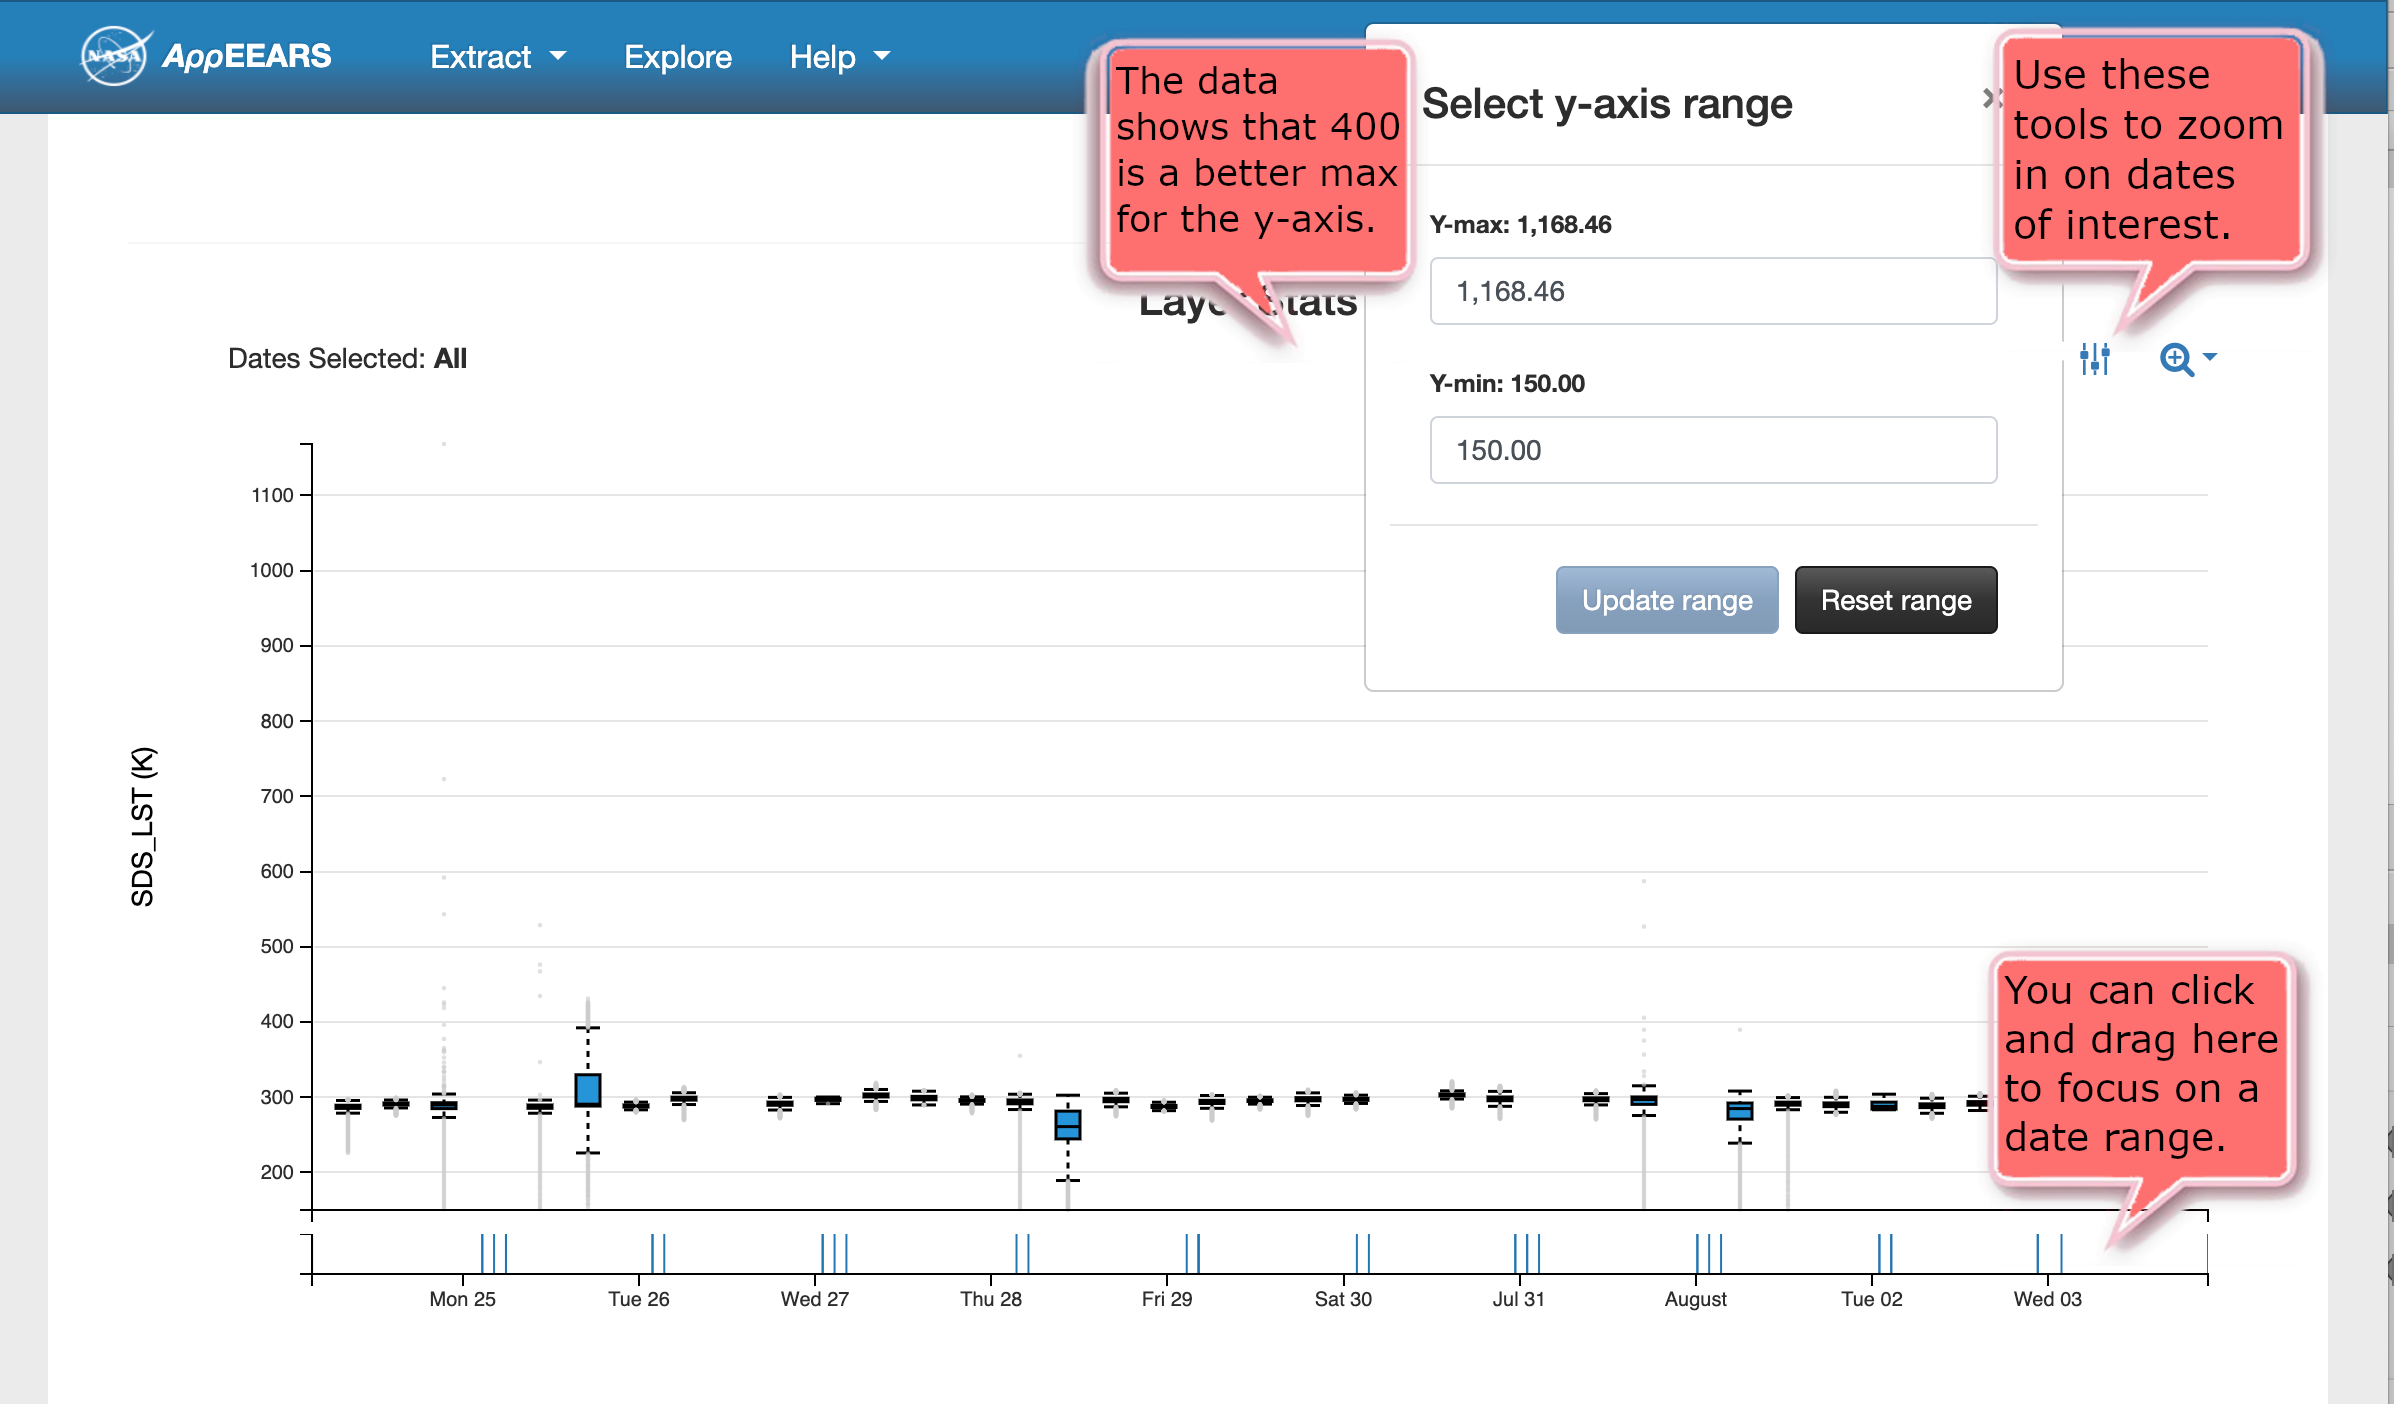
\includegraphics[width=\textwidth]{AppeearsZoom.png}}

	\kulbox{\textbf{NOTE:} It is entirely possible for ECOSTRESS to produce bad data with extreme and unrealistic values for land surface temperature. Make sure you are filtering for clouds. Also, keep in mind that the typical range for surface temperatures varies between -15 $^\circ$F to 115 $^\circ$F. \href{https://doi.org/10.1029/2018GL078133}{Antartica once witnessed frigid temperatures around -145 $^\circ$F} and the \href{https://jeremydforsythe.github.io/icecream-tutorials/Tutorial5_AddingElementsToMaps/Extreme Maximum Land Surface Temperatures.pdf} {theoretical maximum possible ground surface temperature has been estimated to be 212 $^\circ$F.} It is unlikely you will find good quality observations near those extremes for your hometown.}


\section{Temperature Competition Mapping} 

The goal of your map is to quickly and effectively communicate the highest and lowest temperatures for your hometown. With a quick glance the reader should be able to tell:

\begin{enumerate}
	\item Where is your hometown?
	\item When was the highest land surface temperature and how hot did it get?
	\item When was the lowest land surface temperature and how cold was it?
\end{enumerate}

I made an example map using the Vancouver Island shapefile:

\centerline{\includegraphics[width=\textwidth]{Vancouver Island Temperature Competition Example.png}}

Remember too that this is just a bare bones example with just a little personality. We encourage you to make these maps your own. Play around with different basemaps, colors, themes! Just keep in mind that your style choices need to support the science communication goal and not create confusion. For instance, while it might be artistically interesting to use red colors to represent cold temperatures and blue tones for hot temperatures, this will likely confuse your readers as we have become accustomed to the opposite.  

\begin{tcolorbox}[colback=yellow!5!white,colframe=IceCreamLeaf,title=\textbf{Temperature Competition Next Steps}]
	Now that you have that data let's put it all together in a map.
	\begin{enumerate}
		\item Start a new project and load the shapefile for your hometown or favorite place you have lived along with your favorite basemap (Google Satellite, ESRI Imagery, ESRI Delorme, etc,).
		\item Use the same procedures we followed in tutorials \href{https://jeremydforsythe.github.io/icecream-tutorials/Tutorial2_MakingBasicMapsInQGIS/Tutorial2_MakingBasicMapsInQGIS.pdf}{\# 2 Making Basic Maps in QGIS}, \href{https://jeremydforsythe.github.io/icecream-tutorials/Tutorial4_VisualizingDataWithQGIS/Tutorial4_VisualizingDataWithQGIS.pdf}{\# 4 Visualizing Data with QGIS}, \& \href{https://jeremydforsythe.github.io/icecream-tutorials/Tutorial5_AddingElementsToMaps/Tutorial5_AddingElementsToMaps.pdf}{\# 5 Adding Elements To Maps} to create a map with two insets, one for the hottest and coldest days from the 2022 full calendar year using the GeoTIFF files you saved from the previous tutorial. You already have all of the skills to make this map! You don't have to make one that exactly mimics my Vancouver example, but it needs to include all of the design elements that make an effective map: basemap(s), north arrow(s), scalebar(s), title(s), and legend(s). Be curious and creative! Flip through the menus and options!
	\end{enumerate}
\end{tcolorbox}
%%%%%%%%%%%%%%%%%%%%%%%%%%%%%%%%%%%%%%%%%%%%%%%%%%%%%%%%%%%%%%%%%%%%%%%%%%%%%%%%%%% Begin End Matter
	
\vspace{.25em}
	
\hrule

\vspace{1 em}
	
\begin{tcolorbox}[colback=yellow!5!white,colframe=IceCreamOrbit,title= \vspace{.2em} \Large Map of the Week Assignments]
	\addcontentsline{toc}{section}{Map of the Week Assignments}
	\large
	\begin{enumerate}
		\item Submit a map of your hometown (include the boundaries of your shapefile that you used to pull the data from) with two insets, one for the hottest day of the year and the other for the coldest. Use the Vancouver Island map as inspiration, but make the submission your own.  
		\item Include a paragraph describing your map. Think of it as a caption or blurb for a press release. What do you want the reader to know?
	\end{enumerate}	
\end{tcolorbox}
	
\vfill
	
\hrule
	
\vspace{1em}
	
\textbf{Recommended Citation:} Forsythe, J.D., G.R. Goldsmith, and J.B. Fisher. 2023. Observing Earth from Above Tutorials. Chapman University. \url{https://jeremydforsythe.github.io/icecream-tutorials/}
	
\vspace{1em}
	
This work is supported by funding from NASA ECOSTRESS Mission Grant \#80NSSC23K0309 (I.C.E. C.R.E.A.M.: Integrating Communication of ECOSTRESS Into Community Research, Education, Applications, and Media).
	
\end{document}
